\documentclass[a4paper,twoside,10pt]{article}
\usepackage[utf8]{inputenc}
\usepackage{gensymb}
\usepackage{amsmath}
\usepackage{graphicx}
\graphicspath{ {../images/} }

\newcommand{\lbparagraph}[1]{\paragraph{#1}\mbox{}\\}

\newcommand{\eqsp}[1]{\quad\#\quad}

\title{Formelsammlung Physik BMT 14a}
\author{Lukas Dörig, Michelle Meyer, Yan Poblete}
\date{\today\\v1.1}

\begin{document}

\maketitle

\tableofcontents

\pagebreak

\section*{Intro: Geometrie}

\subsection*{Trigonometrie}

\lbparagraph{Generell}

\begin{tabular}{l|l}
    Variable & Beschreibung \\
    \hline
    H & Hypothenuse \\
    GK & Gegenkathete \\
    AK & Ankathete
\end{tabular}

\lbparagraph{Sinus}

\begin{equation}
    \sin{\alpha} = \frac{GK}{H}
    \eqsp{}
    H = \frac{GK}{\sin{\alpha}}
    \eqsp{}
    GK = \sin{\alpha} \times H
\end{equation}

\begin{equation}
    \frac{a}{\sin{\alpha}} = \frac{b}{\sin{\beta}} = \frac{c}{\sin{\gamma}}
\end{equation}

\lbparagraph{Cosinus}

\begin{equation}
    \cos{\alpha} = \frac{AK}{H}
    \eqsp{}
    H = \frac{AK}{\cos{\alpha}}
    \eqsp{}
    AK = \cos{\alpha} \times H
\end{equation}

\begin{gather}
    a^2 = b^2 + c^2 - 2bc \times \cos{\alpha}
    \eqsp{}
    b^2 = a^2 + c^2 - 2ac \times \cos{\beta}
    \\
    c^2 = a^2 + b^2 - 2ab \times \cos{\gamma}
\end{gather}

\lbparagraph{Tangens}

\begin{equation}
    \tan{\alpha} = \frac{GK}{AK}
    \eqsp{}
    AK = \frac{GK}{\tan{\alpha}}
    \eqsp{}
    GK = \tan{\alpha} \times AK
\end{equation}

\lbparagraph{Wechsel- und Stufenwinkel}

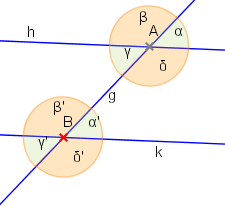
\includegraphics[height=103px,keepaspectratio]{stufen-wechselwinkel}

Wenn h $\parallel$ k. $\alpha$ und $\alpha$' sind Stufenwinkel, $\gamma$ und $\gamma$' sind Wechselwinkel.

%

\section{Kräftegelichgewicht, statisches Gleichgewicht}

\subsection{Koordinaten}

\begin{tabular}{l l}
    Polarform & $(Betrag[F]|Winkel[\alpha])$ \\
    Karthesische Form & $(F_x|F_y)$
\end{tabular}

\lbparagraph{Polar zu Karthesisch}

\begin{equation}
    F_x = F \times \cos{\alpha}
    \eqsp{}
    F_y = F \times \sin{\alpha}
\end{equation}

\lbparagraph{Karthesisch zu Polar}

\begin{equation}
    F = \sqrt{F_x^2 + F_y^2}
    \eqsp{}
    \alpha = \arctan{\frac{F_y}{F_x}} + Sektor
\end{equation}

Für den Sektor muss jeweils addiert werden:

\begin{tabular}{l|l|l|r}
    Sektor & X Positiv? & Y Positiv? & Wert \\
    \hline
    1. & Ja & Ja & $0\degree$ \\
    2. & Nein & Ja & $90\degree$ \\
    3. & Nein & Nein & $180\degree$ \\
    4. & Ja & Nein & $270\degree$
\end{tabular}

\lbparagraph{Vektoren zusammenrechnen (Karthesisch)}

\begin{tabular}{l|l|l}		
  $F_1$ & $F_1x$ & $F_1y$ \\			
  $F_2$ & $F_2x$ & $F_2y$ \\			
  $F_3$ & $F_3x$ & $F_3y$ \\
  \hline
  $F_{res}$ & $F_{res}x$ & $F_{res}y$ \\
\end{tabular}

\subsection{Kräfte}

\begin{tabular}{l|l}
    I & Alle Kräfte heben sich auf \\
    II & Alle Drehmomente heben sich auf
\end{tabular}

\lbparagraph{Im Allgemeinen}

\begin{equation}
    F = m \times a
    \eqsp{}
    [N] = [kg] \times [\frac{m}{s^2}] = [\frac{kg \times m}{s^2}]
\end{equation}

\lbparagraph{Gravitationskraft}

\begin{equation}
    F_{grav} = \frac{G \times m_1 \times m_2}{r^2}
\end{equation}

\lbparagraph{Gewichtskraft}

\begin{equation}
    g = g_{Erde} = 9.81\frac{m}{s^2}
    \eqsp{}
    F_G = m \times g
\end{equation}

\lbparagraph{Hangabtriebskraft}

\begin{equation}
    F_H = F_G \times{\sin{\alpha}}
\end{equation}

\lbparagraph{Normalkraft}

\begin{equation}
    F_N = F_G \times \cos{\alpha}
\end{equation}

\lbparagraph{Reibungkraft}

\begin{equation}
    \mu = [Zahl, 0 - 1]
    \eqsp{}
    F_R = \mu \times F_N
\end{equation}

\lbparagraph{Federkraft}

\begin{equation}
    F_D = k \times x
    \eqsp{}
    F_D = D \times \Delta{s}
    \eqsp{}
    [N] = [\frac{N}{cm}] \times [cm]
\end{equation}

\lbparagraph{Fadenspannung}

\begin{gather}
    T = F_G + F \text{ (Bei hängender Masse)}
    \\
    F = T - F_R \text{ (Bei Masse auf Schiefer Ebene)}
\end{gather}

\subsection{Drehmoment}

\lbparagraph{Generell}

\begin{tabular}{l|l|r}
    Variable & Beschreibung & Einheit \\
    \hline
    M & Drehmoment & [Nm] \\
    $F_{\perp}$ & Kraft, die senkrecht auf die Drehachse wirkt & [N]
\end{tabular}

\begin{equation}
    M = F_{\perp} \times l
\end{equation}

\lbparagraph{Statisch}

\begin{equation}
    F_{1\perp} \times l_1 = F_{2\perp} \times l_2
\end{equation}

\lbparagraph{In Bewegung}

\begin{equation}
    M_{Res} = M_{Uhrzeigersinn} - M_{Gegenuhrzeigersinn}
\end{equation}

\subsection{Flaschenzug und Hebelgesetz}

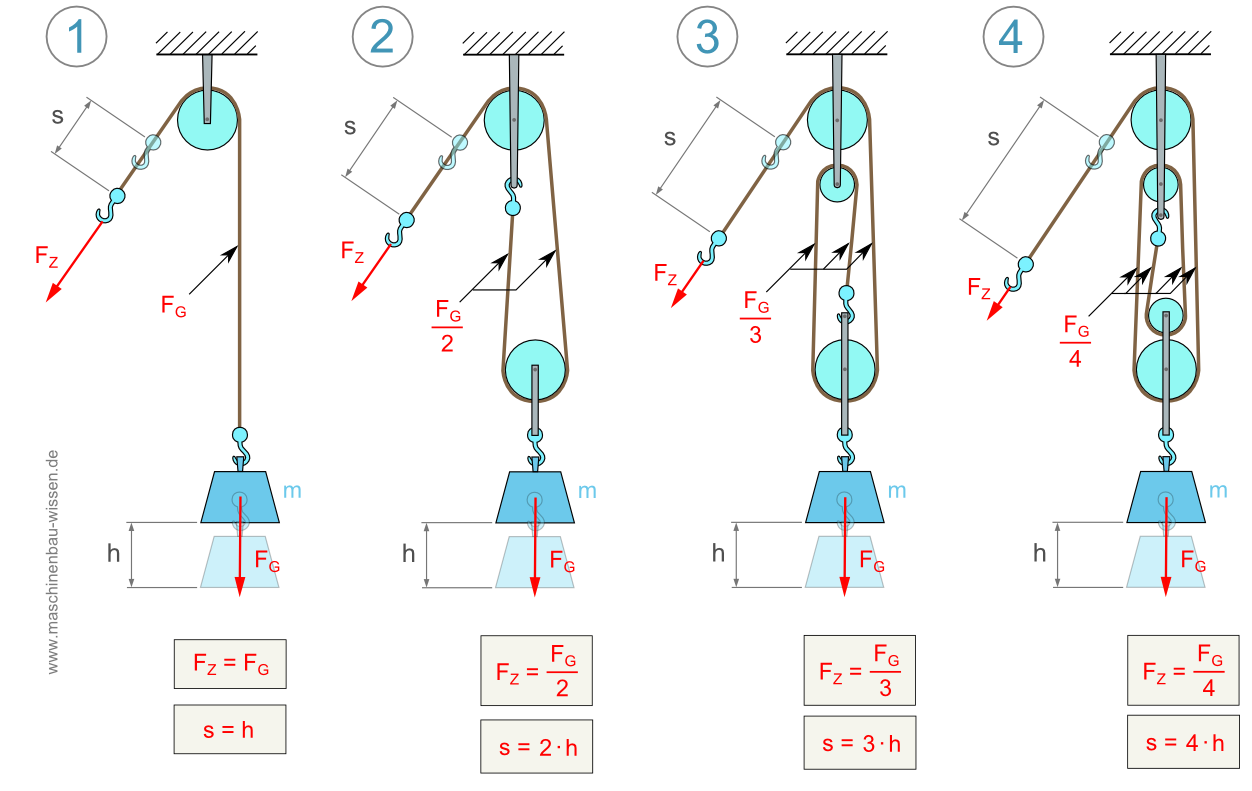
\includegraphics[width=\textwidth,height=\textheight,keepaspectratio]{flaschenzug-berechnen}

\subsection{Hooksches Gesetz}

\lbparagraph{Parallel}

Diese Formeln basieren auf der Annahme, dass parallele Federn sich um dieselbe Distanz strecken.

\begin{gather}
    F = F_1 + F_2
    \\
    D \times s = D_1 \times s + D_2 \times s \qquad | \quad \times\frac{1}{s}
    \\
    D = D_1 + D_2
\end{gather}

\lbparagraph{Seriell}

\begin{equation}
    F = F_1 = F_2
    \eqsp{}
    k = \frac{1}{\frac{1}{k_1} + \frac{1}{k_2}} = \frac{k_1 \times k_2}{k_1 + k_2}
\end{equation}
    
\section{Kinematik, Dynamik (Kraft)}

\subsection{Kinematik}

Hinweis: $v[\frac{km}{h}] = 3.6 \times v[\frac{m}{s}]$ \newline

\begin{tabular}{l|l|l|l}
    Variable & Formeln... & & \\
    \hline
    $\overline{v}$ & $\frac{s}{t}$ & $\frac{v_0 + v}{2}$ & \\
    \hline
    s & $\overline{v} \times t$ & $\frac{v_0 + v}{2} \times t$ & $s_0 + v_0 \times t + \frac{1}{2}a \times t^2$ \\
    \hline
    a & $\frac{v - v_0}{t}$ & & \\
    \hline
    $v^2$ & $v_0^2 + 2as$ & & \\
    \hline
    v & $v_0 + at$ & &
\end{tabular}

\subsection{Drehung}

\lbparagraph{Variablendefinitionen}

\begin{tabular}{l|l|r|r}
    Variable & Beschreibung & Einheit & Weitere Einheiten \\
    \hline
    f & Drehfrequenz & Hz & $[\frac{1}{s}]$ \\
    T & Umlaufzeit & [s] & \\
    n & Anzahl Umdrehungen & [Zahl] &  \\
    b & Bogenlänge & [m] &  \\
    $\theta$ & Drehwinkel & [Radiant] & \\
    $\omega$ & Winkelgeschwindigkeit & $[\frac{1}{s}]$ & $[\frac{Radiant}{s}]$ \\
    $a_z$ & Zentripetalbeschleunigung & $[\frac{m}{s^2}]$ &  \\
    $F_z$ & Zentripetalkraf (=Zentrifugalkraft) & [N] &
\end{tabular}

\lbparagraph{Formeln}

\begin{tabular}{l|l|l|l}
    Variable & Formeln... & & \\
    \hline
    f & $\frac{1}{T}$ & $\frac{n}{\Delta{t}}$ &  \\
    \hline
    $\theta$ & $\frac{b}{r}$ & $\frac{2\pi \times \alpha}{360\degree}$ & $\omega \times t$ \\
    \hline
    $\alpha$ & $\frac{360\degree \times \theta}{2\pi}$ & & \\
    \hline
    $\omega$ & $\frac{\theta}{t}$ & $\frac{v}{r}$ & $2\pi \times f$ \\
    \hline
    v & $\frac{b}{t}$ & $\omega \times r$ & \\
    \hline
    b & $v \times t$ & $\omega \times rt$ & $\theta \times r$ \\
    \hline
    $a_z$ & $\frac{v^2}{r}$ & $\frac{(\omega \times r)^2}{r}$ & $\omega^2 \times r$ \\
    \hline
    $F_z$ & $a_z \times m$ & &
\end{tabular}

\subsection{Keplresche Gesetze}

\paragraph{I}

Die Planeten beschreiben ellipsenförmige Bahnen, in deren einem Brennpunkt die Sonne steht.

\paragraph{II}

Der Radiusvektor $\vec{r}$ überstreicht in gleichen Zeiten gleiche Flächen. $\rightarrow \vec{L} = m \times \vec{r} \times \vec{v} = konstant$

\paragraph{III}

Die Quadrate der Umlaufszeiten zweier Planeten verhalten sich wie die Kuben der grossen Ellipsenhalbachsen:

\begin{equation}
    \frac{T_1^2}{a_1^3} = \frac{T_2^2}{a_2^3}
\end{equation}

\subsection{Bremsweg}

\begin{equation}
    s_b = \frac{V_0^2}{2g\mu} = \frac{v^2 - v_0^2}{-2ab}
\end{equation}

\section{Arbeit, Energie, Leistung}

\subsection{Energieerhaltungssatz}

\lbparagraph{Variablendefinitionen}

\begin{tabular}{l|l|r|r}
    Variable & Beschreibung & Einheit & Weitere Einheiten \\
    \hline
    W & Arbeit & [J] & [Nm]  \\
    E & Energie (gespeicherte Arbeit) & [J] & [Nm] \\
    P & Leistung & [W] & $[\frac{J}{s}] = [\frac{Nm}{s}]$
\end{tabular}

\lbparagraph{Satz}

\begin{equation}
\begin{tabular}{l l l l}
    $E_{tot1}$ & $- E_{Verlust}$ & $+ E_{Zu}$ & $= E_{tot2}$  \\
    $E_{kin1} + E_{pot1} + E_{D1}$ & $- E_R$ & $+ E_{Zu}$ & $= E_{kin2} + E_{pot2} + E_{D2}$
\end{tabular}
\end{equation}

\lbparagraph{Kinetische Energie}

\begin{equation}
    E_{kin} = \frac{1}{2}mv^2
\end{equation}

\lbparagraph{Potentielle Energie}

\begin{equation}
    E_{pot} = mgh
\end{equation}

\lbparagraph{Federenergie \ Deformationsenergie}

D: Federkonstante $[\frac{N}{cm}]$

\begin{equation}
    E_D = \frac{1}{2}Ds^2
\end{equation}

\lbparagraph{Reibungsenergie}

Horizontale:

\begin{equation}
    E_R = F_R \times s = \mu \times mg \times s
\end{equation}

Schiefe Ebene:

\begin{equation}
    E_R = F_R \times s = \mu \times mg \times \cos{\alpha} \times s
\end{equation}

\section{Wärme}

\subsection{Im Allgemeinen}

\lbparagraph{Variablendefinitionen}

\begin{tabular}{l|l|r|r}
    Variable & Beschreibung & Einheit & Weitere Einheiten \\
    \hline
    U & Innere Energie & [J] & \\
    Q & Wärme & [J] & \\
    c & spezifische Wärmekapazität & $[\frac{J}{kg \times K}]$ & \\
    $L_f$ & spezifische Schmelz-/Erstarrungswärme & $[\frac{J}{kg}]$ & \\
    $L_v$ & spezifische Verdampfungs-/Kondensationswärme & $[\frac{J}{kg}]$ & \\
    p & Druck & [Pa] & $[Bar] =10^5 [Pa], [\frac{N}{m^2}]$ \\
    $\vartheta$ & Temperatur in Celsius & $[{\degree}C]$ & \\
    T & Temperatur in Kelvin & [K] &
\end{tabular}

\lbparagraph{STP (Standard Temperature Pressure)}

\begin{equation}
    p_0 = 1.0133
    \eqsp{}
    T_0 = 0{\degree}C = 273.15K 
\end{equation}

\subsection{Änderung Wärme anhand der Temperatur}

\lbparagraph{Wärmemenge}

\begin{equation}
    {\Delta}Q = m \times c \times {\Delta}T
\end{equation}

\lbparagraph{Schmelzwärme}

\begin{equation}
    Q_f = L_f \times m
\end{equation}

\lbparagraph{Verdampfungswärme}

\begin{equation}
    Q_v = L_v \times m
\end{equation}

[???] TODO: Diagramm

\lbparagraph{Wärmeausgleich}

$x_a$ steht für den jeweiligen Aggregatszustand. Um die korrekte Mischtemparatur zu bekommen muss $T_1 < T_2$ sein. Achtung: Man muss Massenänderungen durch Verdampfung einrechnen.

\begin{equation}
    Q_M = Q_1 + {\Delta}Q_1 + Q_{v1} + Q_{f1} = Q_2 + {\Delta}Q_2 + Q_{v2} + Q_{f2}    
\end{equation}

\begin{equation}
\begin{tabular}{ll}
    & $c_1 \times m_1 \times (T_M - T_1) + L_{v1} \times m_{v1} + L_{f1} \times m_{f1}$ \\
    = & $c_2 \times m_2 \times (T_2 - T_M) + L_{v2} \times m_{v2} + L_{f2} \times m_{f2}$
\end{tabular}
\end{equation}

\subsection{Ausdehnung}

\lbparagraph{Bei Gas (Zustandsgleichung ideales Gas)}

Achtung: Nur auf Gase anwenden. Bei Verwendung von STP $p_0...$ anstatt $p_2...$ verwenden.

\begin{equation}
    \frac{p_1 \times V_1}{T_0} = \frac{p_2 \times V_2}{T_2}
\end{equation}

\lbparagraph{Ausdehnung bei festen oder flüssigen Stoffen}

\begin{equation*}
    \alpha, \beta, \gamma = [\frac{1}{K}]
\end{equation*}

\begin{gather}
    {\Delta}l = l_1 - l_0 = \alpha \times l_0 \times {\Delta}T \\
    {\Delta}A = A_1 - A_0 = \beta \times A_0 \times {\Delta}T
    \eqsp{}
    \beta \approx 2 \times \alpha \\
    {\Delta}V = V_1 - V_0 = \gamma \times V_0 \times {\Delta}T
    \eqsp{}
    \gamma \approx 3 \times \alpha
\end{gather}

\subsection{Wärmeleitfähigkeit}

\lbparagraph{Variablendefinitionen}

\begin{tabular}{l|l|r|r}
    Variable & Beschreibung & Einheit & Weitere Einheiten \\
    \hline
    $P_{Th}$ & Thermische Leistung & [W] & $[\frac{J}{s}]$ \\
    k & Wärmeleitfähigkeit & $\frac{W}{m \times K}$ & \\
    A & Querschnittfläche Leiter & $m^2$ & \\
    l & Länge Leiter & m &
\end{tabular}

\lbparagraph{Satz}

\begin{equation}
    P_{Th} = k \times A \times \frac{\vartheta - {\vartheta}_0}{l}
\end{equation}

\end{document}
